%%%%%%%%%%%%%%%%%%%%%%%%%%%%%%%%%%%%%%%%
% 文件名 :     myTemplate.tex          %
%                                      %
% 作者:        包小敏                  %
%                                      %
% 单位:        西南大学数学与统计学院  %\alert{text}
%                                      %
% 创建于:      2011年02月21日          %
% 最后修改于:  2019年11月28日          %
%%%%%%%%%%%%%%%%%%%%%%%%%%%%%%%%%%%%%%%%
\documentclass[x11names,a4paper,AutoFakeBold]{ctexart}
%======================Include Packages========================
\usepackage{SWUthesis}
\usepackage{makecell}
\usepackage{xcolor}
\usepackage{cleveref}%聪明的引用
\usepackage{caption}
\usepackage{bicaption}
\usepackage{threeparttable}
\usepackage{wrapfig}%浮动图片
\usepackage{tasks}%横向列表排版
\usepackage{diagbox}%制作斜线表头
\usepackage{appendix}
%\usepackage{tabularray}

\usepackage{background}
\definecolor{grey}{rgb}{0.91,0.91,0.91}
\SetBgContents{LJW}
\SetBgAngle{-45}
\SetBgColor{grey}
\SetBgOpacity{0.08}
%定义字体
\setCJKfamilyfont{kai}{simkai.ttf}
\crefname{theorem}{定理}{定理} %定义引用标签
\crefname{lemma}{引理}{引理}
\crefname{definition}{定义}{定义}
\crefname{figure}{图}{图}
\crefname{table}{表}{表}
\crefname{algorithm}{算法}{算法}
\renewcommand{\thetable}{\arabic{table}}%改变标题为罗马标签
\renewcommand{\thefigure}{\arabic{figure}}
%设置标题标签和文本字体格式
\captionsetup[table]{labelfont={bf,small },textfont={bf,small},justification=centering}
\captionsetup[figure]{labelfont={bf,small},textfont={bf,small},justification=centering}
\captionsetup[figure][bi-second]{name=Figure} %设置图的英文编号前缀
\captionsetup[table][bi-second]{name=Table} %设置表的英文编号前缀

%\fancyhf{}
\pagestyle{fancy}
\fancyhead[L]{}
\fancyhead[C]{}
\fancyhead[R]{}
\fancyfoot[L]{}
\fancyfoot[C]{\zihao{-5}\small 第\;\thepage\;页\;共\;\pageref*{LastPage}\;页}
\fancyfoot[R]{\tiny\color{grey}LJW}

%%%%%%%%%%%%%%%%%%%%%%%%%%%%%%%%%%%%%%%%%%%%%%%%%%%%%%%%%%%%%%%%
% 指导教师给分及评阅意见
%请在“{}”中填入相应的内容:
%-------------------------------
% 开题意见
\newcommand{\kaitiYN}{同意开题}%也可以填入其它的意见
%===============================
% 评阅日期
\newcommand{\pingyueriqi}{\CJKfamily{kai}\nian 年4月26日}% 请在左边的{}中填入实际的月份和日期
%学习态度
\newcommand{\taidu}{}% 请在左边的{}中填入分数
%设计与撰写水平
\newcommand{\zhuanxie}{}% 请在左边的{}中填入分数
%计算机应用与规范
\newcommand{\jisuanji}{}% 请在左边的{}中填入分数
%科研能力
\newcommand{\keyan}{}% 请在左边的{}中填入分数
%文献整理与分析
\newcommand{\wenxian}{}% 请在左边的{}中填入分数
%研究结果的价值
\newcommand{\jieguo}{}% 请在左边的{}中填入分数
% 评定成绩
\newcommand{\pingdingdengji}{}% 请在左边的{}中填入上面各项分数之和
% 评阅意见
\newcommand{\zcomments}{
	%具体评阅意见在下面填写
	%评阅意见及下面各栏评分项目的得分都在文件夹~{\tt filesforteachers} 中的文件~{\tt zhidaojiaoshigeifen.tex} 内填写。
	%开题报告中的\textcolor{red}{导师意见}也在前述文件内填写(默认意见是:同意开题)。
	\minzi 同学的论文《\biaoti 》立题妥当,描述正确,论述清楚,有一定的实践意义。\\
	本文结构合理,层次分明,思路清晰,显示出作者具有一定的综合运用所学知识的能力,
	符合本科毕业论文的要求,同意其参加论文答辩。见及周边
	%-----------------------------------------------------------------------------
	% 选题(20)
	%\newcommand{\xuanti}{}% 请在左边的{}中填入分数
	%% 能力与态度(40)
	%\newcommand{\nengliyutaidu}{}% 请在左边的{}中填入分数
	%% 质量水平(40)
	%\newcommand{\zhiliangsuiping}{}% 请在左边的{}中填入分数
	%% 论文评定等级
	%\newcommand{\pingdingdengji}{}% 请在左边的{}中填入等级:优、良、合格、不合格
	%% 指导教师评阅分数
	%\newcommand{\jiaoshigeifen}{}
	%% 指导教师评阅分数×0.3
	%\newcommand{\jiaoshiR}{}% ×0.3
	%% 是否同意参加答辩
	%\newcommand{\dabianyn}{同意参加答辩}
	% 指导教师姓名
	%\newcommand{\jiaoshi}{包小敏}
}
% 指导教师评阅及打分
% 交叉评阅教师给分及评阅意见
% 请在“{}”中填入相应的内容:
%------------------------------
% 评阅日期
\newcommand{\jpingyueriqi}{\CJKfamily{kai}\nian 年4月28日}% 请在左边的{}中填入实际的月份和日期
% 选题价值(20)
\newcommand{\jxuanti}{}% 请在左边的{}中填入分数
%计算机应用与规范(15)
\newcommand{\jjisuanji}{}% 请在左边的{}中填入分数
%设计与撰写水平(40)
\newcommand{\jzhuanxie}{}% 请在左边的{}中填入分数
%语言表达(10)
\newcommand{\biaoda}{}% 请在左边的{}中填入分数
%文献整理与分析(15)
\newcommand{\jwenxian}{}% 请在左边的{}中填入分数
% 评定成绩
\newcommand{\jpingdingdengji}{}% 请在左边的{}中填入上面各项分数之和
% 交叉评阅教师姓名
\newcommand{\jiaocha}{交叉评阅教师姓名}% 请在左边{}内填入交叉评阅教师的姓名
%评阅意见
\newcommand{\jcomments}{
	%具体评阅意见在下面填写
	\jiaocha 及交叉评阅意见及下面各栏评分项目的得分都在文件夹~{\tt filesforteachers} 中的文件~{\tt jiaochageifen.tex} 内填写。
	%本论文在立题、阐述过程和所涉知识方面基本符合本科毕业论文的要求,基本观点、所涉知识无错误,
	%完全同意指导教师的评语和给定的成绩。
	%------------------------------------------------------------------------------------------
	%% 能力与态度(40)
	%\newcommand{\jnengliyutaidu}{}% 请在左边的{}中填入分数
	%% 质量水平(40)
	%\newcommand{\jzhiliangsuiping}{}% 请在左边的{}中填入分数
	%% 论文评定等级
	%\newcommand{\jpingdingdengji}{}% 请在左边的{}中填入等级:优、良、合格、不合格
	%% 选题指导思想(10)
	%\newcommand{\sixiang}{}
	%% 选题价值(10)
	%\newcommand{\jiazhi}{}
	%% 选题难度(5)
	%\newcommand{\nandu}{}
	%% 综合运用知识能力(10)
	%\newcommand{\nengli}{}
	%% 文献资料整理与分析能力()
	%\newcommand{\zhengli}{}
	%% 外文运用能力(5)
	%\newcommand{\yingwen}{}
	%% 语言运用能力(5)
	%\newcommand{\yuyan}{}
	%% 计算机运用能力(5)
	%\newcommand{\computer}{}
	%% 毕业论文撰写水平(30)
	%\newcommand{\xiezuo}{}
	%% 规范化程度(10)
	%\newcommand{\guifandu}{}
	%% 交叉评阅分数
	%\newcommand{\jiaochageifen}{}
	%% 交叉评阅分数×0.3
	%\newcommand{\jiaochaR}{}% ×0.3
}
      % 交叉评阅及打分
% 答辩分数、等级及评审意见
% 请在“{}”中填入相应的内容:
%------------------------------
%% 答辩分数
%\newcommand{\dabian}{}
%% 答辩分数×0.4
%\newcommand{\dabianR}{}  % ×0.4
%% 论文成绩
\newcommand{\thesisGrade}{合格} % 论文成绩
% 论文评定等级
\newcommand{\dabiancj}{88}    % 答辩成绩
% 答辩评审意见
\newcommand{\dcomments}{
	% 具体评审意见在下面填写
	评审意见及下面的论文评定等级都在文件夹~{\tt filesforteachers} 中的文件~{\tt dabianchengji.tex} 内填写。
	%\minzi 同学的论文《\biaoti 》立题合理,具有一定的实践意义,所涉知识符合本科毕业论文的要求。
	%在答辩中叙述清楚,有条理,能正确回答所提问题,答辩态度认真,状态良好。
	%----------------------
}
      % 答辩成绩
%%%%%%%%%%%%%%%%%%%%%%%%%%%%%%%%%%%%%%%%%%%%%%%%%%%%%%%%%%%%%%%%
\makeindex%生成索引
%===========================请填入相应的内容===================%
\newcommand{\university}{西南大学}                             %
\newcommand{\school}    {数学与统计学院}                       %
\newcommand{\city}      {重庆 400715}                          %
\newcommand{\biaoti}{毕业论文模板}                 % 中文论文题目。如题目太长,可把一部分放在副标题的位置
\newcommand{\cobiaoti}{附带说明}                  % 副标题,没有的话将“---附带简单的使用说明”删除
\newcommand{\enbiaoti}{Undergraduate Thesis {\LaTeX} Template} % 英文论文题目
\newcommand{\nianji}  {2018 级}                                % 年级
\newcommand{\zhuanye}{统计学}                  % 专业
\newcommand{\minzi}{{\CJKfamily{kai}李嘉伟}}                   % 学生中文姓名
\newcommand{\englishname}{Name of Student}                     % 学生英文姓名
\newcommand{\jiaoshi}{\CJKfamily{kai}李婷婷}                   % 指导教师姓名
\renewcommand{\jiaocha}{{\CJKfamily{kai}交叉评阅教师}}         % 请在左边{}内填入交叉评阅教师的姓名
\newcommand{\xuehao}{\CJKfamily{kai}222018314210017}           % 学号
\newcommand{\nian}{\CJKfamily{kai}2020}                        % 毕业年份
\newcommand{\nianxian}{十四}                                   % 已使用年数(=2019-2006)
\newcommand{\kaitiriqi}{\CJKfamily{kai}2019年12月20日}         % 开题日期
\newcommand{\tijiaoriqi}{\CJKfamily{kai}\today}                % 提交日期
\newcommand{\dayinriqi}{\CJKfamily{kai}\today}                 % 打印日期
%===============================================================
% 若修改过程中某个文件不需修改,则将\includeonly中这个文件名注释掉可以加快编译速度。
% 请用PDFLATEX编译,直接生成PDF文件。也可用 LATEX 编译,但速度可能会非常慢,有时甚至可能会出错。
%===============================================================
\includeonly{tables/coverpage,
             tables/pingyue_1,
             tables/pingyue_2,
             tables/dabian,
             biaoge/kaiti_1,
             biaoge/kaiti_2,
             fulu
}
%======================
\makeindex

\begin{document}
\begin{titlepage}
\begin{center}
	%要学校的logo时使用此封面头
	%    \begin{tabular}{cc}
		%        
\includegraphics[width=3cm]{preample/xishilogo.eps}
		%        &
		%        \raisebox{8.6ex}[0pt]{
			%        \begin{tabular}{c}
				%        
\includegraphics[height=1.3cm,angle=0]{preample/xishi.eps}\\\\
				%
				%        {\textbf{\zihao{1} 本科毕业论文(设计)}}
				%    \end{tabular}}\\
		%\end{tabular}
		%不要学校的logo时使用此封面头
		\begin{tabular}{c}
			
\includegraphics[height=1.3cm,angle=0]{preample/xishi.eps}\\\\
			
			\hspace{.8cm}{\textbf{\zihao{1} 本科毕业论文(设计)}}
		\end{tabular}
		%-------------------------------------------------
	\end{center}
	\vspace{2.0cm}
	
	\huge\zihao{2}
	\begin{tabular}{ll}
		{\textbf{题\quad 目}}& \biaoti \\\cline{2-2}
		&\cobiaoti\\
	\end{tabular}
	\vspace{2.4cm}
	
	\begin{center}
		\begin{tabular}{rrllc}
			\huge\zihao{3}{\textbf{学}} & & & \huge\zihao{3}{\textbf{院}} & {\huge\zihao{3}{\CJKfamily{kai}\school}}\\\cline{5-5}
			\huge\zihao{3}{\textbf{专}} & & & \huge\zihao{3}{\textbf{业}} & {\huge\zihao{3}{\CJKfamily{kai}\zhuanye}}\\\cline{5-5}
			\huge\zihao{3}{\textbf{年}} & & & \huge\zihao{3}{\textbf{级}} & {\huge\zihao{3}\nianji}\\\cline{5-5}
			\huge\zihao{3}{\textbf{学}} & & & \huge\zihao{3}{\textbf{号}} & {\huge\zihao{3}\xuehao}\\\cline{5-5}
			\huge\zihao{3}{\textbf{姓}} & & & \huge\zihao{3}{\textbf{名}} & {\huge\zihao{3}\minzi}\\\cline{5-5}
			\huge\zihao{3}{\textbf{指}} & \huge\zihao{3}{\textbf{导}} & \huge\zihao{3}{\textbf{教}}&\huge\zihao{3}{\textbf{师}}& {\huge\zihao{3}\jiaoshi}\\\cline{5-5}
			\huge\zihao{3}{\textbf{成}} & & & \huge\zihao{3}{\textbf{绩}} & {\huge\zihao{3}{\CJKfamily{kai}\thesisGrade}}\\\cline{5-5}
		\end{tabular}
		\vspace{3.2cm}
		
		{\LARGE\zihao{3}\dayinriqi}
	\end{center}

\end{titlepage}
%====================生=成=目=录===================================
%%%%%%%%%%%%%%%%%%%%%%
\pagenumbering{roman}%
\thispagestyle{plain}%
%%%%%%%%%%%%%%%%%%%%%%
\tableofcontents
\thispagestyle{plain}
\newpage
%==========================摘要===================================
%%%%%%%%%%%%%%%%%%%%%%%%
\pagenumbering{arabic} %
\setcounter{page}{1}   %
%%%%%%%%%%%%%%%%%%%%%%%%
\begin{center}
{\heiti\bf\LARGE\zihao{3}{\biaoti\cobiaoti}}

\vspace{0.3cm}
{\zihao{-4}\minzi}

{\zihao{5}\university\school,\city}
\end{center}
\addcontentsline{toc}{section}{摘要}
\begin{center}
\begin{minipage}[t]{13cm}
\noindent{\zihao{5}{\bf 摘要:}
\fangsong
%%%%%%%%%%%%%%%%%%%%%%%%%%%%%%%%%%%%%%%%%%%%%%%%%%%%%%%%%%%%%%%%%%%%%%%%%%%%%%%%%%%%%%%%//
% 请填入中文摘要:
本模版是为{\university\school}本科毕业生而设计的,
模版根据{\school}论文的Word模版中所描述的要求编写。目的是简化和
规范学位论文的撰写,使得论文作者可以将精力集中到论文的内容上而不是浪费在版面设置上。
使用者只需了解{\LaTeX}的基本概念即可使用本模版。

}\vspace{0.1cm}

\noindent{\songti\zihao{5}{\bf 关键词:} \LaTeX ;模版;论文;版面;参数
%%%%%%%%%%%%%%%%%%%%%%%%%%%%%%%%%%%%%%%%%%%%%%%%%%%%%%%%%%%%%%%%%%%%%%%%%%%%%%%%%%%%%%%%%%
}\vspace{0.6cm}
\end{minipage}
\end{center}
\begin{center}
{\Large\bf\zihao{4}\enbiaoti}

\vspace{0.3cm}
{\normalsize\zihao{5}\englishname}

{\small School of Mathematics \& Statistics, Southwest University,Chongqing 400715}
\end{center}
\addcontentsline{toc}{section}{Abstract}
\noindent{\normalsize\zihao{5}{\bf Abstract:}
%%%%%%%%%%%%%%%%%%%%%%%%%%%%%%%%%%%%%%%%%%%%%%%%%%%%%%%%%%%%%%%%%%%%%%%%%%%%%%%%%%%%%%%%%//
% 请填入英文摘要:
This {\LaTeX} template is designed for the undergraduate students of
the School of Mathematics and Statistics at the Southwest
University. The design of the template followed the undergraduates
thesis requirements described in the Word templates. Our purposes
are to reduce the editing workload for the students, standardize the
layout of their theses. Only basic knowledge of the {\LaTeX} is
required to use this template.

}\vspace{0.1cm}

\noindent{\normalsize\zihao{5}{\bf Key words:} {\LaTeX};template;thesis;layout;parameters}
%\end{minipage}
%\end{center}

%=======================正文开始==================================
\large\zihao{-4}
%---------------------------------------
\section{关于模板的一些说明}%\label{chpt:1}
%---------------------------------------
本模版\glossary{模板}是为{\university\school}本科毕业生撰写毕业论文而设计的,版面尺寸按照{\school}的论文撰写要求选取。模板的第一版是
2006年完成的,经过多年的使用、 改进,最终发展成目前的版本。

第一次使用本模版时,请先阅读~\ref{subsec:1}节;如果安装\CTeX{}\index{\CTeX}有问题,请阅读~\ref{sec:versionSelect}节;如果对数学公式、符号或定义、定理、证明等各种命令环境不熟悉,请阅读第~\ref{sec:2two}
节;如果对表格或图形的\index{图形插入}插入不熟悉,请阅读第~\ref{sec:ssss}节;如果对\index{交叉引用}交叉引用\index{交叉引用}不熟悉,请阅读第~\ref{sec_si4}节。 如果想了解在~\LaTeX 中\index{程序引入}引入程序代码,如
~{\tt Matlab},{\tt Mathematica},{\tt R} 和~{\tt C/C++} 等的代码,请阅读第~\ref{sec:codeinludsion}节并分别参考附录~\ref{appendix:A}、~\ref{appendix:B}、~\ref{appendix:C}、\ref{appendix:D} 中的实例。
\subsection{模板的构成}\label{subsec:1}
本模板由若干文件组成,所有文件都存放在一个主文件夹\index{文件夹}里。为了使用和管理方便,在主文件夹中又分了五个子文件夹:{\tt codes, biaoge, filesforteachers, preample, tables},其中~{\tt preample\index{文件夹!preample}, tables\index{文件夹!table}} 中的文件一般不用管,
而~{\tt codes\index{文件夹!codes}} 在熟悉模板后可以删除。文件夹~{\tt biaoge\index{文件夹!biaoge}} 包含一些由学生填写的表格文件,而文件夹~{\tt filesforteachers\index{文件夹!filesforteachers}} 则包含一些由教师填写的表格文件(当然也可由学生复制进去)。模板由主文件~{\tt mytemplate.tex\index{mytemplate.tex}} 及五类子文件构成:
\begin{enumerate}
	\item 论文的编译通过主文件才能进行。学生的基本信息,如姓名,学号,论文题目等,都在主文件上输入。
	\item\label{item:2} 这一类文件是论文的主要组成部分,由学生完成。有以下几个文件:
	\begin{enumerate}
		\item {\tt abstract.tex\index{abstract.tex}},这是论文的摘要。
		\item {\tt body.tex\index{body.tex}},这是论文的正文部分。
		\item {\tt bibfile.tex\index{bibfile.tex}},这是论文的参考文献。
		\item {\tt thanks.tex\index{thanks.tex}},这是论文的致谢词部分。
	\end{enumerate}
	以上两类文件都存放在主文件夹里,学生只须在相关的文件中按~\LaTeX\index{\LaTeX} 的要求及文件中的提示输入相应的内容即可。
	%\item 这一类是三个与教师有关的文件:
	%\begin{enumerate}
	%  \item\label{term1} {\tt zhidaojiaoshigeifen.sty},这个文件包含指导教师评分及评阅意见,由指导教师完成。
	%  \item {\tt jiaochageifen.sty},这个文件包含交叉评阅意见及评分,由负责交叉评阅的教师完成。
	%  \item {\tt dabianchengji.sty},这个文件包含答辩评审意见、答辩分数及论文成绩,由教师答辩小组组长完成。
	%\end{enumerate}
	%这类文件存放在子文件夹~{\tt filesforteachers} 中。相关教师只须在对应的文件中按\LaTeX
	%的要求及文件中的提示输入相应的内容即可。具体的对应文件及填写方法参看后面表格(开题报告二~\pageref{table:kaiti_2},教师评阅表~\pageref{table:pingyue},交叉评阅表%~\pageref{table:jiaochapingyue},答辩记录表~\pageref{table:dabianjilu})中的说明。
	\item 这一类有四个文件:
	\begin{enumerate}
		\item {\tt kaiti\_1.tex\index{kaiti\_1.tex}}(开题报告一);
		\item {\tt kaiti\_2.tex\index{kaiti\_2.tex}}(开题报告二);
		%\item {\tt renwu.tex}(任务书);
		\item {\tt dabianjilu.tex\index{dabianjilu.tex}}(答辩记录)。
	\end{enumerate}
	这类文件存放在子文件夹~{\tt biaoge} 中。前两个文件是开题报告,最后一个文件是答辩记录。完成人只须在对应的文件中按~\LaTeX 的要求及文件中的提示输入相应的内容即可。
	具体的对应文件及填写方法参看后面表格(第~\pageref{table:kaiti_1} 页开题报告一,第~\pageref{table:kaiti_2} 页开题报告二,第~\pageref{table:dabianjilu} 页答辩记录表)中的说明。
	\item\label{item:4} 这一类是三个与教师有关的文件:
	\begin{enumerate}
		\item\label{term1} {\tt zhidaojiaoshigeifen.tex\index{zhidaojiaoshigeifen.tex}},这个文件包含指导教师评分及评阅意见,由指导教师完成。
		\item {\tt jiaochageifen.tex\index{jiaochageifen.tex}},这个文件包含交叉评阅意见及评分,由负责交叉评阅的教师完成。
		\item {\tt dabianchengji.tex\index{dabianchengji.tex}},这个文件包含答辩评审意见及论文评定成绩,由教师答辩小组组长完成。
	\end{enumerate}
	这类文件存放在子文件夹~{\tt filesforteachers} 中。相关教师只须在对应的文件中按~\LaTeX
	的要求及文件中的提示输入相应的内容即可。具体的对应文件及填写方法参看后面表格(第~\pageref{table:kaiti_2} 页开题报告二,第~\pageref{table:pingyue} 页指导教师评阅表,第~\pageref{table:jiaochapingyue} 页交叉评阅表
	,第~\pageref{table:dabianjilu} 页答辩记录表)中的说明。
	\item\label{item:head} 这一类中除头文件{ \tt SWUthesis.sty\index{SWUthesis.sty}} 外还有一些诸如学校的~logo 和学院的~logo 之类的文件。
	这几个文件单独放在子文件夹~{\tt preample} 中,这些文件一般不用改动。
	
	%这四类文件在前面相关的内容录入后,通过编译主文件,会自动将指导教师评阅意见,交叉评阅意见以及答辩记录,答辩分数和论文等级等相关的内容导入对应表格,最后生成~PDF 格式的文件。
	\item\label{item:miscellanceous} 这一类中有四个文件:{\tt coverpage.tex\index{coverpage.tex}}(封面),{\tt pingyue\_1.tex\index{pingyue\_1.tex}}(指导教师评阅表), {\tt pingyue\_2.tex\index{pingyue\_2.tex}} (交叉评阅表),
	{\tt dabian.tex}(答辩记录表)。这几个文件,单独放在子文件夹~{\tt tables} 中,它们只生成封面或表格的框架,其中需要填入的内容通过编译会自动从其它相关文件中导入,
	所以一般不用对这些文件做改动。
\end{enumerate}
总之第~\ref{item:head} 类和第~\ref{item:miscellanceous} 类的文件一般不用去管,主文件和~\ref{item:2}--~\ref{item:4} 类中的子文件在完成后由学生统一通过主文件编译,
最后生成包含所有内容和所有表格的、完整的论文的~PDF 格式的文件。子文件夹~{\tt codes} 中放有一些制作本说明时所用的一些文件,如果不需要可以删除。
\subsubsection{三级标题}
本节为测试三级标题在目录中的显示而设。
\subsection{\CTeX{} 简介}
\TeX{} 是计算机科学家、图灵奖得主~Knuth\index{Knuth} 教授设计的一款权威的科技论文排版软件!学习~\TeX(\LaTeX),
Knuth 的专著~\cite{knuth} 无疑是权威之选。该书排版堪称完美,从中可以看出大师的魅力。更重要的是~Knuth 教授无偿公开了~\TeX{} 的所有源代码,
也就是说它是开源 (Open Source)的(通俗地说就是可以免费使用)。正因为这个原因,后人在其基础上开发了~\LaTeX 。\LaTeX{} 方便好用,被广泛传播,成了当今世界科技界最权威的论文排版软件。
作为一个非常全面的~\LaTeX{} 的参考书,\cite{companion} 是一个不错的选择。如果阅读英文有困难,作为一个初学者,也可以先看看~\cite{zhanglibo}。

\TeX{} 和~\LaTeX{} 排版软件和~MS 的~Word 软件不同,后者是``所见即所得\index{所见即所得}"(WYSIWYG\index{WYSIWYG},what you see is what you get),而前者是``所想即所得\index{所想即所得}"(WYWIWYG\index{WYWIWYG},what you want is what you get)。
二者在风格上迥然不同,因此学习~\LaTeX{} 需要稍微改变一下自己的习惯。

%\paragraph{Run-in headings.}
目前国内使用的~\LaTeX{} 汉化版\index{\LaTeX{} 汉化版}称为~
\CTeX ,最新的版本为~2.9.2.164,可在~\href{http://www.ctex.org/HomePage}{\CTeX{} 网站}~\index{\CTeX 网站}免费下载安装。
\subsection{\CTeX{} 的安装\index{\CTeX 的安装}}\label{sec:versionSelect}
根据我个人及我指导过的 \nianxian 届学生的使用经历,2.4.5-8 版的\CTeX (安装文件是\\{\tt
	CTeX-2.4.5-8-Full.exe})在~XP 操作系统下的问题较少,占用空间也较小,因此在~XP 操作系统下我推荐使用这个版本的~\CTeX。但在安装时要先把安装计算机上的时间调到较早的一个时间,
如$2004$年,待安装完毕运行一次后再将时间调回当前时间,否则运行时会报错。在~Win 7 或以上的操作系统下,安装~2.4.5-8 版的~\CTeX{} 可能会出现问题;而安装最新版的~
2.9.2.164(安装文件为~
CTeX~\_2.9.2.164\_Full.exe)时,DVI 阅读器~{\tt YAP}\index{YAP} 可能会报错。只需按提示点击弹出窗口相应的按钮继续安装。安装好后,如果用{ \tt LATEX} 编译,打开~DVI 文件时可能会频繁弹出
恼人的{ \tt MiKTeX Problem Report} 错误报告窗口。这个问题发生的原因我目前在网上还没有看到合理的解释,当然也没有发现有人给出过解决方法。估计发生的原因可能和操作系统有关。
通过反复琢磨和测试,我找到一个解决办法,就是在~DVI 窗口
进入{ \tt View --> Options...},这时会弹出{ \tt Options} 窗口,点击{ \tt Display},在{ \tt Default render} 右端下拉菜单中有两个选项(见图~\ref{fig:optionWin}):{\tt Pk} 和{ \tt Dvips},
选择{ \tt Dvips}作为默认值后问题即可解决。其它版本的~\CTeX{} 若出现类似地问题也可这样来解决。我在~\CTeX\_2.9.0.152 版上测试过,
用这个方法解决了同样的问题。
\begin{figure}
	\centering
	% Requires \usepackage{graphicx}
	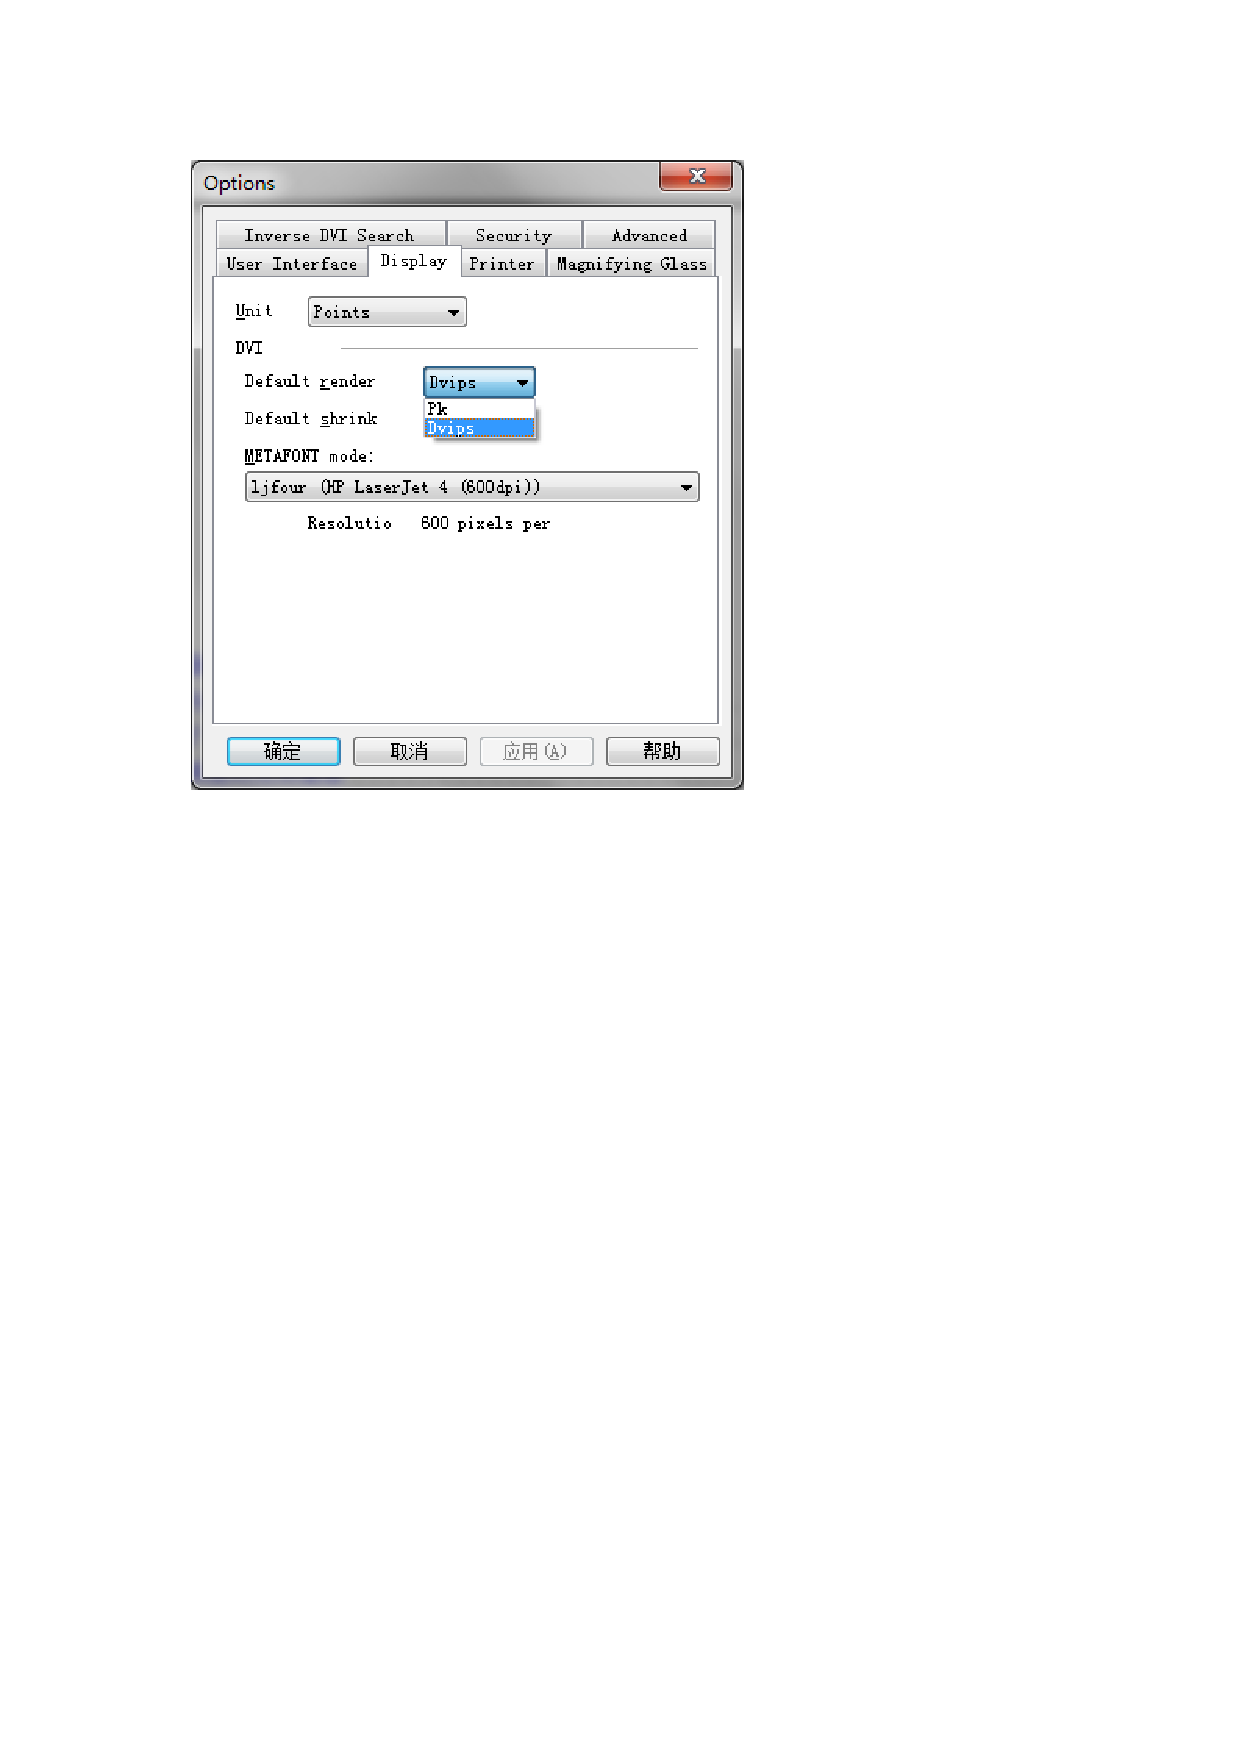
\includegraphics[width=8cm]{codes/292164wenti}\\
	\caption{{\tt Options} 窗口}\label{fig:optionWin}
\end{figure}
%---------------------------------------
\subsection{\CTeX{} 文件的编译\index{\CTeX 文件的编译}}
%---------------------------------------
在新版~\CTeX$2.9.2.164$ 下,一般情况下用{ \tt PDFLateX} 编译,直接生成PDF文件。也可用{ \tt LATEX} 编译,但速度可能会非常慢,有时甚至可能会出错。

如果用{ \tt PDFLateX} 编译后生成的PDF没有自动打开,那么就在{ \tt WinEdt} 编辑窗口的顶端点击{ \tt Options},在下拉菜单中选择{ \tt Execution Modes...},再在弹出的窗口中的第一栏中选择{ \tt PDFLaTex},在第二栏中勾选{ \tt Start Viewer}(如图~\ref{fig:optionPDF}),然后点击{ \tt OK}收起窗口,之后再编译即可。
\begin{figure}
	\centering
	% Requires \usepackage{graphicx}
	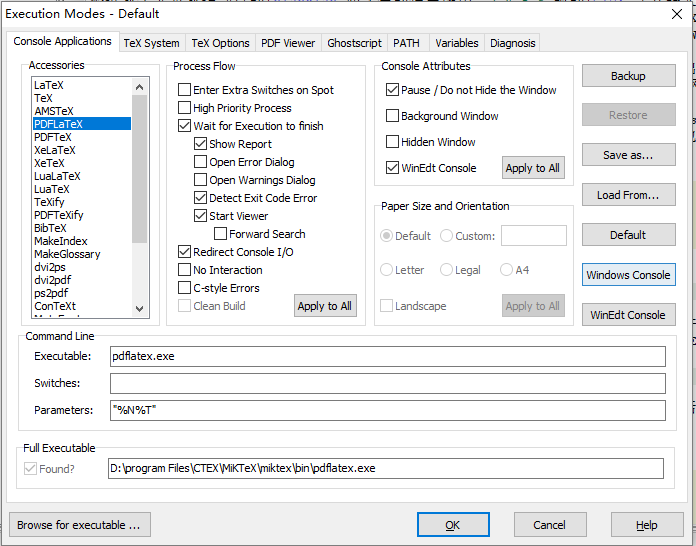
\includegraphics[width=16cm]{options.png}\\
	\caption{编译后自动打开PDF文件的设置}\label{fig:optionPDF}
\end{figure}

%---------------------------------------
\subsection{书签的选择\index{书签}}
%---------------------------------------
新版\CTeX$2.9.2.164$默认的{\rm PDF}阅读器\index{PDF阅读器}是~{\rm sumatraPDF\index{sumatraPDF}}。有时成功编译后(需编译两次),{\rm sumatraPDF} 打开的{\rm PDF} 文件左端并没有书签。这时只须点击{\tt 查看}(如图~\ref{fig:bookmarkselection}),
在下拉菜单中点击{\tt 书签},书签即可出现。
\begin{figure}
	\centering
	% Requires \usepackage{graphicx}
	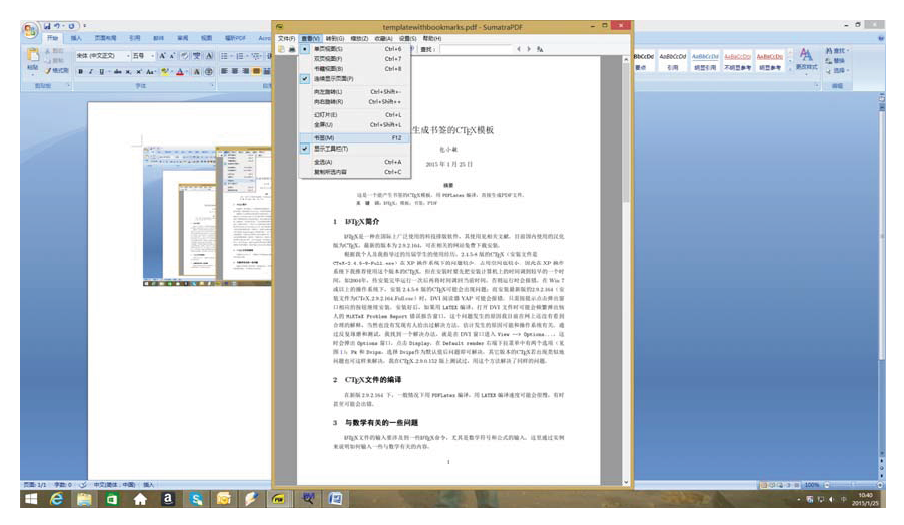
\includegraphics[width=16cm]{codes/selectbookmarks.eps}\\
	\caption{书签的选择}\label{fig:bookmarkselection}
\end{figure}
%---------------------------------------
\subsection{索引的生成\index{索引的生成}}
%---------------------------------------
学院对本科生的毕业论文并没有要求索引,但如果有人想给出索引,那么可以按下面步骤来生成索引:
\begin{enumerate}
	\item 对文章中需要列入索引的词组(如索引)的后面输入\verb=\index{索引}=;
	\item 在主文件中将\%\verb=\makeindex= 前的\%去掉;
	\item 在主文件{ \tt myTemplate.tex} 的编辑窗口上端点击{ \tt TeX},在下拉菜单中点击{\tt Make~Index}(见图~\ref{fig:gensuoyin}),然后再点击{ \tt PDFLaTeX} 编译即可。
\end{enumerate}
\begin{figure}
	\centering
	% Requires \usepackage{graphicx}
	\includegraphics[width=8cm]{gensuoyin.jpg}\\
	\caption{生成索引的操作}\label{fig:gensuoyin}
\end{figure}

%---------------------------------------
\subsection{\CTeX{} 文件编译后产生的附属文件}
%---------------------------------------
%\begin{figure}
%  \centering
%  % Requires \usepackage{graphicx}
%  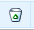
\includegraphics[width=2cm]{garbagecan.png}\\
%  %\caption{}\label{}
%\end{figure}
\CTeX{} 文件的编译会产生一些附属的文件,如后缀为{\tt .aux,.idx,.log,.out}的文件。在最后的PDF文件编译完成后,如果想删除这些文件,可以点击{\rm WinEdt}窗口上部~GUI 中的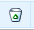
\includegraphics[width=.4cm]{garbagecan.png},在弹出的窗口中点击``OK"(见图~\ref{fig:deletewin})即可将相应的文件删除。
\begin{figure}
	\centering
	% Requires \usepackage{graphicx}
	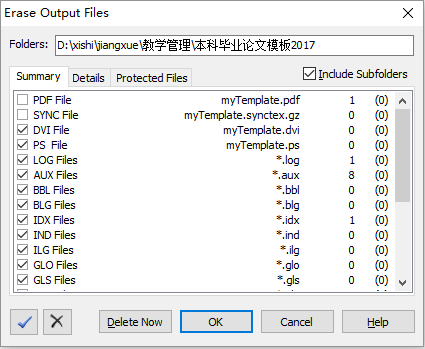
\includegraphics[width=8cm]{deletewin.png}\\
	\caption{删除附属文件的窗口}\label{fig:deletewin}
\end{figure}

%---------------------------------------
\section{与数学有关的一些内容}\label{sec:2two}
%---------------------------------------
\subsection{常见的数学环境\index{数学环境}示例\index{数学环境}}
\LaTeX 文件的输入要涉及到一些 \LaTeX 命令,尤其是数学符号和公式的输入。这里通过实例来说明如何输入一些与数学有关的内容。建议学生在使用前阅读一遍。通过对比PDF文件中的效果和源文件对应的排版命令,初学者可以快速上手使用\LaTeX 。
\begin{definition}
	设
	\begin{equation}\label{eq:1}
		a_1,a_2,\cdots, a_n, \cdots
	\end{equation}
	是一个数列。和
	$$\sum_{i=1}^n a_i$$
	称为数列~\eqref{eq:1} 的前$n$项和。
\end{definition}
\begin{lemma}[新定理]
	若$p$是一个素数,且$p$不能够被$a\in \mathbb{N}$整除,则
	$$a^{p-1}\equiv 1\pmod{p}.$$
\end{lemma}
\begin{proof}
	引理的证明在此给出。
\end{proof}
\begin{theorem}[欧拉定理\index{欧拉定理}]\label{thm:euola}
	若$\gcd(a,n) = 1$,则
	$$a^{\phi(n)}\equiv 1\pmod{n}.$$
\end{theorem}
\begin{proof}
	下面我们来证明这个定理。
\end{proof}
\begin{lemma}[费尔马小定理\index{费尔马小定理}]
	若$p$是一个素数\index{素数},且$p$不能够被$a\in \mathbb{N}$整除,则
	$$a^{p-1}\equiv 1\pmod{p}.$$
\end{lemma}
\begin{proof}
	引理的证明在此给出。
\end{proof}
\begin{corollary} 由组合数的定义立得
	$$\binom{n}{k}=\binom{n}{n-k}.$$
\end{corollary}
\begin{property}
	性质的内容。
\end{property}
\begin{example}[2011\ 江苏卷]在平面直角坐标系$xOy$中,$M$,$N$分别是椭圆$C$:
	$\frac{x^{2}}{4^{2}}+\frac{y^{2}}{2^{2}}=1$的顶点,
	过坐标原点的直线交椭圆于$P$,$A$两点,其中点$P$在第一象限.过$P$ 作$x$轴的垂线,
	垂足为$C$.连接$AC$,并延长交椭圆与点$B$.设直线$PA$的斜率为$k$.\\
	\parbox{10cm}{
		\begin{enumerate}
			\item 若直线$PA$平分线段$MN$,求$k$的值;
			\item 当$k=2$时,求点$P$到直线$AB$的距离$d$;
			\item 对任意的$k>0$,求证:$PA\perp PB$.
	\end{enumerate}}
	\parbox{3cm}{
		\begin{center}
			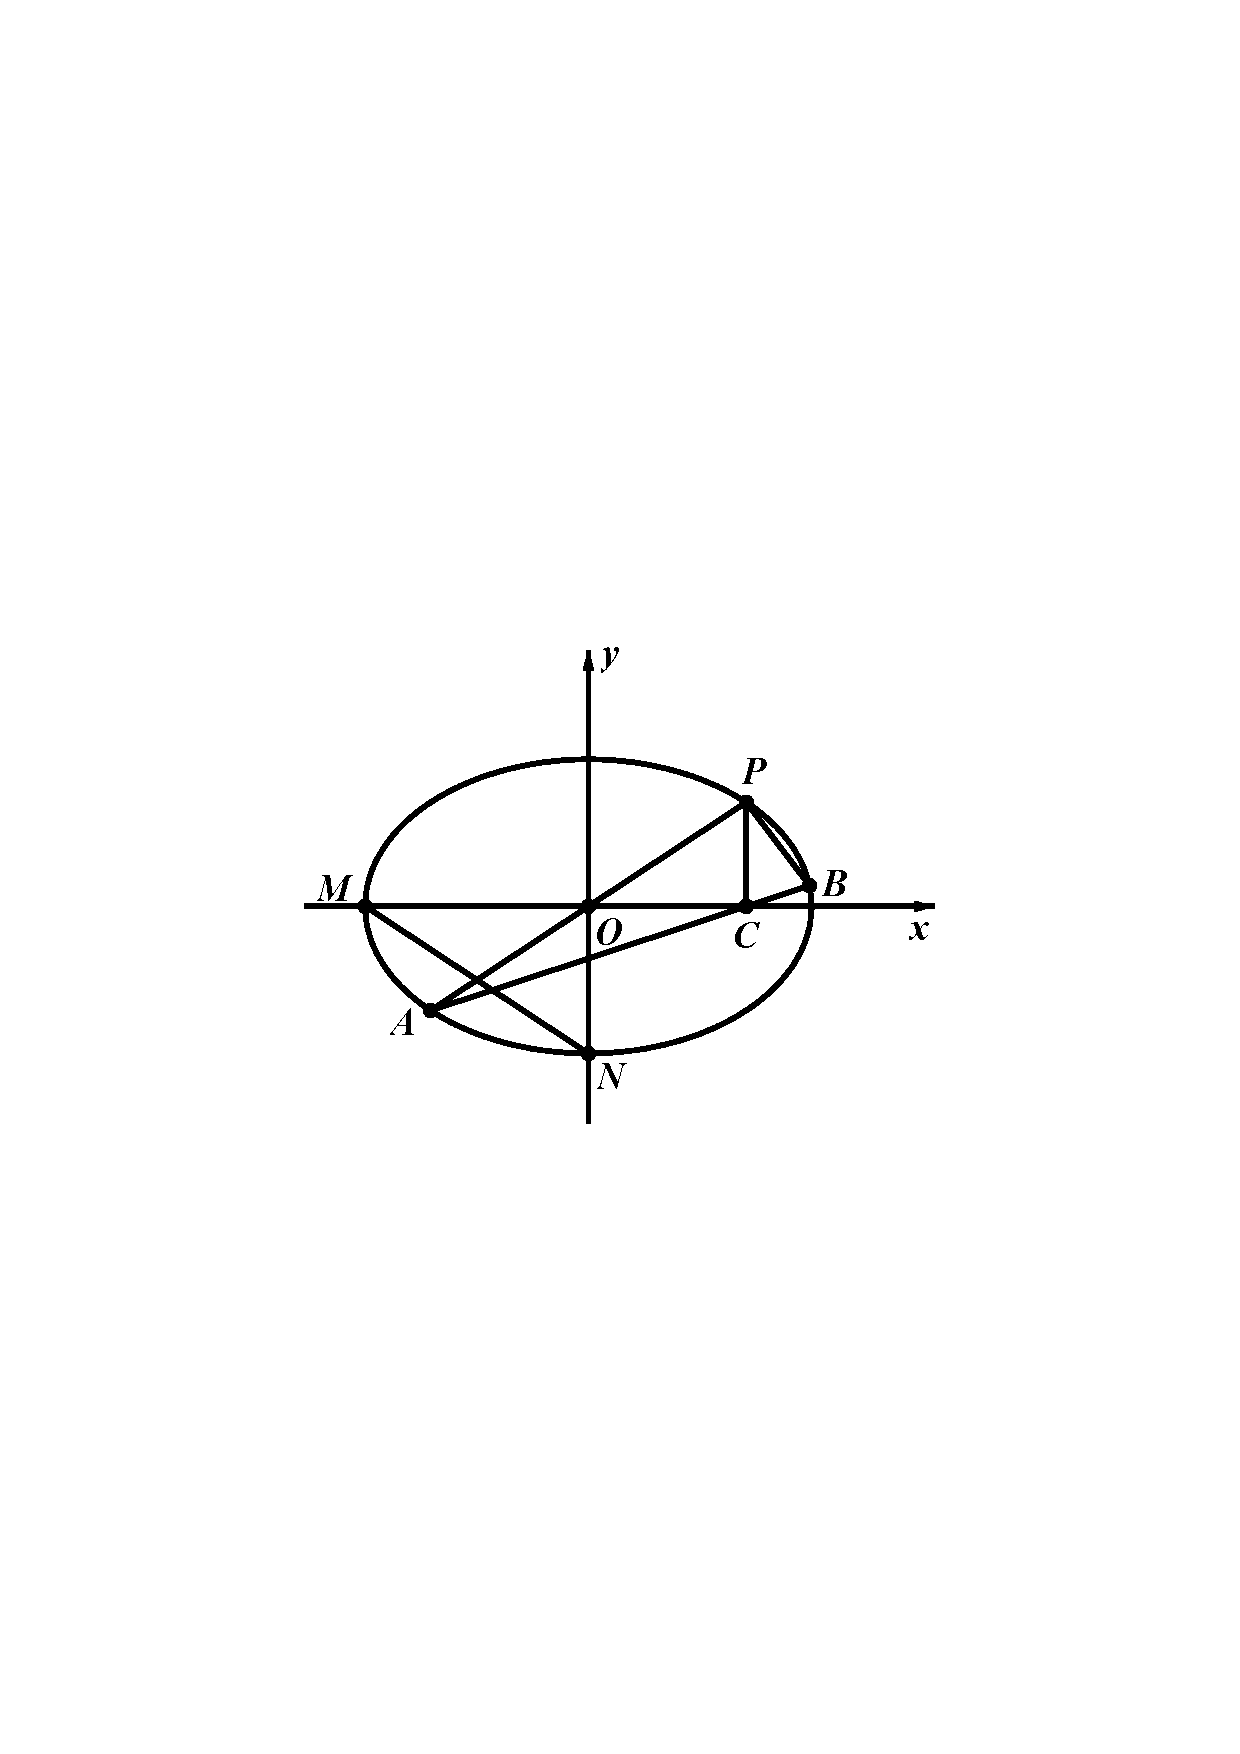
\includegraphics[height=3cm,angle=0]{wangyang_2.pdf}\\
			%\caption{椭圆}\label{fig:1}
	\end{center}}
\end{example}

\begin{example}[2010,重庆卷]
	例题的内容$\langle ID,\mu,\gamma\rangle$,$\langle ID,\mu,\gamma\rangle$。
\end{example}
\begin{solution}
	解答的内容。
\end{solution}
\begin{exercise}
	练习题的内容。
\end{exercise}
\begin{note}
	注释的内容。
\end{note}
\begin{proposition}
	命题的内容。
\end{proposition}
\begin{proof}
	命题的证明。
\end{proof}

\subsection{算法的排版\index{}}
用\CTeX 可以排出版面非常漂亮的算法\index{算法的排版}。根据所用宏包的不同,所用的命令也有所不同。下面是用宏包~{\tt algorithm} 和~{\tt algorithmic} 进行算法排版的一个例子。所排的算法是著名的\index{欧几里得算法}欧几里得算法\citeu{stinson}。

%%%%%%%%%%%%%%%%%%%%%%%%%%%%%%%%%%%%%%%%%%%%%%%
\begin{algorithm}
	\caption{Euclidean algorithm$(a,b)$}
	\label{alg:euclid}
	\algsetup{indent=2em}
	\begin{algorithmic}[1]
		\REQUIRE 整数$a,b\ne 0$
		\ENSURE  商序列$q_1,q_2,\cdots,q_m$和$\gcd(a,b)$
		\STATE $r_0 \leftarrow a$
		\STATE $r_1 \leftarrow b$
		\STATE $m\leftarrow 1$
		\WHILE{$r_m\ne 0$}
		\STATE $q_m\leftarrow\lfloor\frac{r_{m-1}}{r_m}\rfloor$
		\STATE $r_m\leftarrow r_{m-1}-q_mr_m$
		\STATE $m\leftarrow m+1$
		\ENDWHILE
		\STATE $m\leftarrow m-1$
		\RETURN {$(q_1,q_2,\cdots, q_m;r_m)$}
		\STATE {\bf{comment:}$r_m = \gcd(a,b)$ }
	\end{algorithmic}
\end{algorithm}
算法~\ref{alg:euclid_no}是另一个标号\index{算法标号}的。
\begin{algorithm}
	\caption{Euclidean algorithm$(a,b)$}
	\label{alg:euclid_no}
	\algsetup{indent=2em}
	\begin{algorithmic}[2]
		\REQUIRE 整数$a,b\ne 0$
		\ENSURE  商序列$q_1,q_2,\cdots,q_m$和$\gcd(a,b)$
		\STATE $r_0 \leftarrow a$
		\STATE $r_1 \leftarrow b$
		\STATE $m\leftarrow 1$
		\WHILE{$r_m\ne 0$}
		\STATE $q_m\leftarrow\lfloor\frac{r_{m-1}}{r_m}\rfloor$
		\STATE $r_m\leftarrow r_{m-1}-q_mr_m$
		\STATE $m\leftarrow m+1$
		\ENDWHILE
		\STATE $m\leftarrow m-1$
		\RETURN {$(q_1,q_2,\cdots, q_m;r_m)$}
		%\STATE {\bf{comment:}$r_m = \gcd(a,b)$ }
	\end{algorithmic}
\end{algorithm}

%\setcounter{algorithm}{4}
下面的算法~\ref{alg:rgg}是一个生成$q$进制$n$元反射Gray码\index{反射Gray码}的算法。
\begin{algorithm}
	\caption{\sc Reflected Gray Code Generation$(q, n)$}
	\label{alg:genGraycode}
	\algsetup{indent=2em}
	\begin{algorithmic}
		%%\TitleOfAlgo{Euclidean algorithm$(a,b)$}
		\label{alg:rgg}
		\REQUIRE{整数$q>0,n > 0$}
		\ENSURE {$q^n\times n$矩阵$G$}
		\STATE $g_{n-1}g_{n-2}\cdots g_{0}\longleftarrow 00\cdots 0$
		\WHILE{$(2\mid q$ \AND $g_{n-1},g_{n-2},\cdots ,g_{0} \neq q-1,\bm{0}_{n-1})$ \OR $(2\nmid q$ \AND $g_{n-1},\cdots ,g_{n} \neq \bm{(q-1)}_{n}$}
		\STATE $i\leftarrow 0$
		\STATE $\sigma \leftarrow (g_{n-1}+g_{n-2}+\cdots +g_{i+1})\bmod 2$
		\IF{$\sigma=0$ \AND $g_{i}\neq q-1$}
		\STATE $g_{i} \leftarrow g_{i}+1$
		\ELSIF{$\sigma =1$ \AND $g_{i}\neq 0$}
		\STATE $g_{i}\leftarrow g_{i}-1$
		\ENDIF
		\STATE $i \leftarrow i+1$
		\IF{$i = q-1$}
		\STATE $g_{i} \leftarrow g_{i}+1$
		\ENDIF
		\ENDWHILE
	\end{algorithmic}
\end{algorithm}
%再来一个不标号不连线的:
%\LinesNotNumbered
%\SetAlgoNoLine
%
%\begin{procedure}[H]
%\caption{$f$()\hspace{-.15cm}$(x,a,b)$}
%\label{proc:f}
%\KwIn{$x,a,b$}
%\uIf{$x\in S_1$}{
	%    $f\leftarrow (\beta x,a,(b+1)\bmod n)$
	%    }
%\uElseIf{$x\in S_2$}{
	%    $f\leftarrow (x^2,2a\bmod n,2b\bmod n)$
	%    }
%\Else{
	%    $f\leftarrow (\alpha x,(a+1)\bmod n,b)$
	%    }
%\Return{$(f)$}
%\end{procedure}
\begin{algorithm}
	%\COMMENT{external}% {\bf  External: }}
%\begin{algorithmic}
\caption{{\sc Collision-To-Second-Preimage}\,$(h)$}
\label{algo:c2sec}
\begin{algorithmic}
	%\REQUIRE{Hash 函数$h$}
	\STATE \bf{External: }{\sc Oracle-2nd-Preimage}
	\STATE Choose $x\in_R\mathcal{X}$
	\IF{{\sc Oracle-2nd-Preimage}\,$(h,x) = x'$}
	\RETURN $(x,x')$
	\ELSE{\RETURN{{\rm(``failure")}}}
	\ENDIF
\end{algorithmic}
\end{algorithm}
%---------------------------------------
\section{多栏排版\index{多栏排版}}
%---------------------------------------
多栏环境是一个常用的环境,下面是一个两栏排版的例子。
\begin{Parallel}[v]{0.38\textwidth}{}
\ParallelLText{在最早的
	中国求圆学者
	中,必须首先
	要提到的是张
	衡。他是汉朝
	的一位著名科
	学家。}
\ParallelRText{Among the earliest
	Chinese circle-squarers
	mention must be made
	of Chang Heng in the
	first p1ace. He was a famous
	scholar of the Han
	Dynasty.}
\end{Parallel}
%---------------------------------------
\section{表格、公式与插图\index{插图}}\label{sec:ssss}
%---------------------------------------
\subsection{表格}
%---------------------------------------

%$$\sum_{i=1}^m(-1)^i\binom{m+n-i}{i,m-i,n-i} = \sum_{i=1}^m(-1)^i\binom{m}{i}\binom{m+n-i}{m}, \mbox{其中$m\leq n$}$$


表题应写在表格\index{表格}上方正中,表序写在表题左方不加标点,空一格写表题,表题末尾不加标点,全文的表格统一编序,表序必须连续。
\begin{table}[h]
\centering
\caption{一些数学符号的{\LaTeX}输入命令与效果对照表}\label{table:1}
\begin{tabular}{|c|c|}\hline
	输入 & 输出 \\\hline
	\verb=$(\sum x_{ij})^{1/p}$= & $(\sum x_{ij})^{1/p}$ \\\hline
	\verb=$\left(\sum x_{ij}\right)^{1/p}$= & $\left(\sum x_{ij}\right)^{1/p}$ \\\hline
	\verb=$\bigl(\sum x_{ij}\bigr)^{1/p}$= & $\bigl(\sum x_{ij}\bigr)^{1/p}$ \\\hline
	\verb=$\Bigl(\sum x_{ij}\Bigr)^{1/p}$= & $\Bigl(\sum x_{ij}\Bigr)^{1/p}$ \\\hline
	\verb=$\biggl(\sum x_{ij}\biggr)^{1/p}$= & $\biggl(\sum x_{ij}\biggr)^{1/p}$ \\\hline
	\verb=$\Biggl(\sum x_{ij}\Biggr)^{1/p}$= & $\Biggl(\sum x_{ij}\Biggr)^{1/p}$ \\
	\hline
\end{tabular}
\end{table}
表题用五号宋体居中(见表~\ref{table:1}),表格内中文用五号宋体,英文用五号Times
New Roman字体。

表题允许下页接写,接写时表题省略,表头应重复书写,并在右上方写``续表xx"。下面是一些表格的实例。
%\begin{table}
%\tbl{Radio-band beaming model parameters for\\ {FSRQs and BL Lacs.}}
%{\begin{tabular}[l]{@{}lcccccc}
	%\toprule
	%  Class$^{\rm a}$ & $\gamma _1$ & $\gamma _2$$^{\rm b}$
	%
	%         & $\langle \gamma \rangle$
	%
	%         & $G$ & $|{\bm f}|$ & $\theta _{c}$ \\
	%
	%\hline%colorrule
	%  BL Lacs &5 & 36 & 7 & $-4.0$ & $1.0\times 10^{-2}$ & 10$^\circ$ \\
	%  FSRQs & 5 & 40 & 11 & $-2.3$ & $0.5\times 10^{-2}$ & 14$^\circ$ \\
	%\bottomrule
	%\end{tabular}}
	%\tabnote{$^{\rm a}$This footnote shows what footnote symbols to use.}
	%\tabnote{$^{\rm b}$This footnote shows the text turning over when a long footnote is added.}
	%\label{symbols}
	%\end{table}
	
	%\taburulecolor | gray!50|{red} \arrayrulewidth=1pt
	%{
		%\taburulecolor | yellow |{blue}
		%\begin{tabu}{|X|X|} \hline
		%Here the lines & are drawn in blue \\ \taburulecolor {green} \hline
		%But starting from here & they are green coloured ! \\ \hline
		%And now a nested tabu & \begin{tabu}{X} \firsthline\hline
			%guess what colour \\ \hline
			%is used for rules ?\\ \lasthline \hline
			%\end{tabu} \\\hline
			%\end{tabu}
			%In side the group, rule colors are blue
			%}%
		%After the group, rule colors are red again !
		%\begin{tabu}{X}\hline \hline \indent \end{tabu}
		
		
		\begin{table}[htb]
			\centering\caption{三线表示例}
			\begin{tabular}{ccccc}\toprule
				姓名 & 平时成绩 & 期中考试 & 期末考试 & 最后成绩\\\midrule
				张三 & 60       & 78       & 76       & 67      \\
				李四 & 89       & 92       & 98       & 95      \\
				王五 & 95       & 91       & 100      & 97      \\\bottomrule
			\end{tabular}
		\end{table}
		\begin{center}
			\begin{tabular}{|c|c|c|c|c|c|c|c|}\hline
				\multirow{2}*{题号} & \multicolumn{5}{c|}{第一部分} & \multirow{2}*{第二部分} & \multirow{2}*{总分}\\\cline{2-6}
				& 一 & 二 & 三 & 四 & 五        &                         & \\\hline
				得分 &    &    &    &    & $\surd$   &                         & \\\hline
			\end{tabular}
		\end{center}
		\begin{table}[htb]
			\centering
			\caption{一班课程表}
			\begin{tabular}{|c| *{7}{c|}}\hline
				\backslashbox{课节}{星期} & 星期一 & 星期二 & 星期三 & 星期四 & 星期五 & 星期六 & 星期日 \\\hline
				1 & & & & & & &  \\\hline
				2 & & & & & & &  \\\hline
				3 & & & & & & &  \\\hline
				4 & & & & & & &  \\\hline
				5 & & & & & & &  \\\hline
				中午& \multicolumn{7}{c|}{}   \\\hline
				6 & & & & & & &  \\\hline
				7 & & & & & & &  \\\hline
			\end{tabular}
		\end{table}
		%---------------------------------------
		\subsection{公式}
		%---------------------------------------
		公式应另起一行,正文中的公式\index{公式}、算式或方程式等应编排序号,公式的编号用圆括号括起,
		序号标注于该式所在行(当有续行时,应标注于最后一行)的行末。公式可按章节顺序编号或按全文统一编号。公式序号必须连续,
		不得重复或跳缺。重复引用的公式不得另编新序号。
		较长的公式,如必须转行时,最好在等号处转行,如做不到这一点,要在$+,
		-, \times, \div$等数学符号处转行。
		数学符号应写在转行处的行首。上下式尽可能在等号``="处对齐。
		$\sum\limits_{i=1}^nn^2$
		
		\begin{flushleft}
			$
			\begin{aligned}
				f(x,y) &= f(0,0) + \frac{1}{1!}\left(x\frac{\partial}{\partial x}+y\frac{\partial}{\partial y}\right)f(0,0) \\
				&= \frac{1}{2!}\left(x\frac{\partial}{\partial x}+y\frac{\partial}{\partial y}\right)^2f(0,0) + \cdots\\
				&= \frac{1}{n!}\left(x\frac{\partial}{\partial x}+y\frac{\partial}{\partial y}\right)^nf(0,0) + K
			\end{aligned}
			$
		\end{flushleft}
		
		\[
		\begin{aligned}
			f(x,y) &= f(0,0) + \frac{1}{1!}\left(x\frac{\partial}{\partial x}+y\frac{\partial}{\partial y}\right)f(0,0) \\
			&= \frac{1}{2!}\left(x\frac{\partial}{\partial x}+y\frac{\partial}{\partial y}\right)^2f(0,0) + \cdots\\
			&= \frac{1}{n!}\left(x\frac{\partial}{\partial x}+y\frac{\partial}{\partial y}\right)^nf(0,0) + K
		\end{aligned}
		\]
		\begin{equation}\label{eq:a}
			\begin{split}
				f(x,y) =& f(0,0) + \frac{1}{1!}\left(x\frac{\partial}{\partial x}+y\frac{\partial}{\partial y}\right)f(0,0) \\
				& + \frac{1}{2!}\left(x\frac{\partial}{\partial x}+y\frac{\partial}{\partial y}\right)^2f(0,0) + \cdots\\
				& + \frac{1}{n!}\left(x\frac{\partial}{\partial x}+y\frac{\partial}{\partial y}\right)^nf(0,0) + K
			\end{split}
		\end{equation}
		\[ \Set{x\in\mathbf{R} | 0<|x|<\frac{5}{3}} \]
		\[
		\left\{\vphantom{\frac{5}{3}}x\in\mathbf{R} \right/\left.
		0<{|x|}<\frac{5}{3}\right \}
		\]
		$$S = \sum_{i=1}^n m_i$$
		\[\left\{
		\begin{aligned}
			a_{11}x + a_{12}y &= b_1 \\
			a_{21}x + a_{22}y &= b_2
		\end{aligned}
		\right.
		\]
		方程组只要一个编号
		\begin{equation}
			\begin{aligned}
				a_{11}x + a_{12}y &= b_1 \\
				a_{21}x + a_{22}y &= b_2\\
				a_{21}x + a_{22}y &= b_2
			\end{aligned}
		\end{equation}
		或者
		\begin{equation}
			\left\{
			\begin{aligned}
				a_{11}x + a_{12}y &= b_1 \\
				a_{21}x + a_{22}y &= b_2
			\end{aligned}
			\right.
		\end{equation}
		方程组中如每个方程要单独编号,则可写成
		\begin{numcases}{}
			%要使用cases package
			a_{11}x + a_{12}y = b_1\label{eq:111} \\
			a_{21}x + a_{22}y = b_2\label{eq:222}
		\end{numcases}
		\eqref{eq:111}-\eqref{eq:222}
		或
		\begin{align}
			a_{11}x + a_{12}y &= b_1 \\
			a_{21}x + a_{22}y &= b_2
		\end{align}
		
		\[
		f(x) =  \left\{
		\begin{array}{ll}
			x+1, & \hbox{if $x>1$;} \\
			-x, & \hbox{if $x\leq 1$.}
		\end{array}
		\right.
		\]
		%---------------------------------------
		\makeatother
		\subsection{插图}
		每幅插图\index{插图}应有图序和图题,全文插图可以统一编序,图序必须连续,不得重复或跳缺。
		图序和图题写在图的下方(见图~\ref{fig:1}),五号宋体居中。
		\begin{figure}
			\centering
			
\includegraphics[height=6.6cm,angle=0]{preample/ms}\\
			\caption{数学与统计学院院徽}\label{fig:1}
		\end{figure}
		下面是两种图片并列(图~\ref{fig:33} 和图~\ref{fig:44},图~\ref{fig:21}和图~\ref{fig:22})的两种情形:
		\begin{figure}[b]
			\centering
			\begin{minipage}[t]{5cm}
				\centering
				\mbox{\resizebox{!}{35mm}{
\includegraphics{preample/ms}}}\\
				\caption{数学与统计学院院徽}\label{fig:33}
			\end{minipage}
			\hspace{1.5cm}
			\begin{minipage}[t]{5cm}
				\centering
				\mbox{\resizebox{!}{15mm}{
\includegraphics{preample/xishi}}}\\
				\caption{西南大学}\label{fig:44}
			\end{minipage}
		\end{figure}
		
		%%%%%%%%%%%%%%%%%%%%%%%%%%%%%%%%
		\begin{figure}
			\centering
			\mbox{\subfigure[第一个子图]{\resizebox{!}{15mm}{
						
\includegraphics{preample/xishi}\label{fig:21}
			}}}\hspace{1.5cm}
			\mbox{\subfigure[第二个子图]{\resizebox{!}{35mm}{
						
\includegraphics{preample/ms}\label{fig:22}
			}}}\\
			\caption{西南大学}
		\end{figure}
		%---------------------------------------
		\section{参考文献的引用\index{引用}示例}\label{sec_si4}
		%---------------------------------------
		按论文中参考文献出现的次序,用中括号的数字连续编号,五号宋体,文献顶格,单倍行距(见例~\ref{li:2})。引用格式按照西南大学学报要求,
		请注意标点符号。
		国内高等院校数学专业常用的两本\citeu{xiong,zhang}《近世代数》是张禾瑞编著的
		《近世代数》\cite{zhang}和熊全淹编著的 《近世代数》\cite{xiong}.
		\begin{example}\label{li:2}
			参考文献中条目排版示例:
			\begin{verbatim}
				[4] 郑霖,柴宗新,郑远昌等.四川省地理[M].四川科学技术出版社,
				1994.108-111.
				[5] 刘广珠. 高中生考试焦虑成因分析[J].陕西师大学报(哲社版),
				1995,24(1):161-164.
			\end{verbatim}
		\end{example}
		这是一个外文参考文献的引用实例\citeu{experqc}。请注意上面两种引用格式,一种是上标, 一种是正常。使用者可根据自己的喜好选用。
		
		这是另外一种引用方式~\cite{das},如果必要也可以这样用。
		
		
		\section{程序代码的插入\index{代码的插入}}\label{sec:codeinludsion}如果论文涉及到较长的计算机程序,可以考虑将其放在附录中。使用下面的命令
		\begin{verbatim}
			\lstinputlisting[language=代码语言]{代码文件名}
		\end{verbatim}
		即可将程序代码引入~\CTeX 中,这里``代码语言"是指编写代码所使用的语言,如~{\tt C/C++},{\tt Matlab} 等,而``代码文件名"是指存放代码所使用的文件名(如代码文件存放在与 fulu.txt 不同的文件夹中,
		还需给出那个文件夹的路径)。附录~\ref{appendix:A}---\ref{appendix:D}\index{附录}
		给出了~{\tt C/C++},{\tt Matlab},{\tt Mathematica} 和~{\tt R} 的具体例子。
		

%=======================参考文献=================================%
\renewcommand{\baselinestretch}{\yuanbeishu} %
\normalsize\zihao{5}                         %
%\vspace{1cm}                                %
\addcontentsline{toc}{section}{参考文献}     %
\begin{thebibliography}{9}                   %
%\vspace{.4cm}
%%%%%%%%%%%%%%%%%%%%%%%%%%%%%%%%%%%%%%%%%%%%%%%%%%%%%%%%%%%%%%%%%%
\bibitem{moban_1}
    西南大学数学与统计学院.
    \textsl{本科毕业论文(设计)规范化要求(论文最新模版)}.
\bibitem{tongzhi}
    西南大学数学与统计学院.
    \textsl{关于2017届本科毕业论文工作安排的通知}.
\bibitem{experqc}
    C.H.Bennett, F.Bessette, G.Brassard, et al,
    \textsl{Experimental quantum cryptography} [J].
    Journal of Cryptology, Vol.5, No.1(1992), 3--28.
\bibitem{latex}
    \TeX\, Guru.
    \textsl{\LaTeX 2e 用户手册}. 1999.
\bibitem{knuth}
    Donald E. Knuth,
    \textsl{The \TeX book} [M]. Addison-Wesley, 1984.
\bibitem{knuth_2}
    Donald E. Knuth,
    \textsl{The Arts of Computer Programming} [M]. 北京:机械工业出版社, 2008.
\bibitem{stinson}
    D. R. Stinson,
    \textsl{Cryptography---Theory and Practice (Third Edition)}[M]. Chapman \& Hall/CRC, Taylor \& Francis Group, Roca Raton, FL, USA. 164.
\bibitem{xiong}
    熊全淹,
    \textsl{近世代数} [M]. 武汉大学出版社, 1995年.
\bibitem{companion}
    Frank Mittelbach, Michel Goossens.
    \textsl{The \LaTeX \,Companion (Second Edition)}[M]. Addison-Wesley, 2005.
\bibitem{zhanglibo}
    张林波等.
    \textsl{CCT中外文科技排版系统} [M].北京:海洋出版社,1993年。
\bibitem{zhang}
    张禾瑞,
    \textsl{近世代数} [M].高等教育出版社, 1978年.
\bibitem{das}
    Das,M.L., Saxena, A., and Phatak,D.B.
    \emph{Algorithms and Approaches of Proxy Signature: A Servey}. arXiv:cs/0612098v1 [cs.CR],20 Dec 2006. ~\href{https://arxiv.org/pdf/cs/0612098.pdf}{https://arxiv.org/pdf/cs/0612098.pdf.}

\end{thebibliography}

%=========================索引===================================%
\printindex %如不要索引请将此行和下行注释掉
\addcontentsline{toc}{section}{索引}
%=========================致谢===================================%
%%%%%%%%%%%%%%%%%%%%%%%%%%%%%%%%%%%%%%%%%%%%%%%%%%%%%
\renewcommand{\baselinestretch}{\beishu}\normalsize %
%%%%%%%%%%%%%%%%%%%%%%%%%%%%%%%%%%%%%%%%%%%%%%%%%%%%%
%\noindent\large\zihao{-4}{\bf 致谢:}
\section*{致谢:}%\label{endofThesis}
\addcontentsline{toc}{section}{致谢}
%-----------------------------------
本模板目前的版本是由2006年完成的初始版经多年反复修改而来。西南大学数学与统计学院前后几十位同学在使用过程中所反馈的意见
是本模板发展的强大推动力。在此我要感谢所有使用过模板的同学,尤其是模板完成后最初几年使用过的同学,他们承受了初期模板中存在
的问题所带给他们的种种不便,有时甚至可能是痛苦。同时我也要感谢数学与统计学院的领导和某些老师对使用本模板的宽容态度,
正是由于他们的宽容,才使得本模板的使用和推广成为可能。我还要特别感谢我的同事彭作祥教授多年来的热情鼓励以及一些有益的建议,
他在2014年将模板推荐给统计系$2015$届的同学使用,从而使更多的同学开始接触到\LaTeX 和\CTeX 。自2016年以来,学院就``建议所有学生的毕业论文(设计)均使用latex模板排版"\citeu{tongzhi},
我本人当然欢迎更多的同学使用我这个模板。

希望大家在使用~\CTeX 编辑完成论文后能体会到当年~D.E.Knuth 教授在修订他的长篇巨著《The Arts of Computer Programming》\cite{knuth_2} 时还不得不抽出大量的时间来设计、
研制\LaTeX 的前身\TeX 的心情,以及\LaTeX 对当今社会的影响。同时我更希望~\CTeX 能给大家今后的工作、学习和生活带来更多的便利。

由于~\LaTeX 一直在不断的更新,同时计算机的操作系统也在不断升级,再加上本人也是一个业余的~\LaTeX 爱好者,水平有限,因此模板难免会有这样或那样的问题。请将问题或者建议~email 告诉我,我的~email
地址是~\href{mailto:xbao@swu.edu.cn}{\tt xbao@swu.edu.cn}。

\vspace{2cm}

\begin{center}
    \begin{tabular}{cp{3cm}l}
         &   & {\minzi}   \\
         &   & {\tijiaoriqi~\Printtime}   \\
         &   & {于\university~25 教~1520 } \\
     \end{tabular}
\end{center}
%\label{endofThesis}

%=========================附录===================================%
\begin{appendix}
%\begin{appendix}
\section{Matlab 代码} \label{appendix:A}

下面是我写的一个~Matlab
代码,这个代码可以给出下面这个
1989年第30届国际数学奥林匹克(IMO)竞赛的一道试题的一个解答:\vspace{.5cm}

\noindent 求证:集合$\Set{1, 2,
\cdots,1989}$可以分为$117$个互不相交的子集
$$A_i, \qquad i = 1, 2, \cdots,117$$
使得
\begin{enumerate}
    \item 每个$A_i$都含有$17$个元素;
    \item 每个$A_i$中所有元素之和相同。
\end{enumerate}\vspace{.5cm}

这个代码的文件名为~{\tt equalsumpartition.m},运行时在~Matlab 命令窗口键入下面的命令
\begin{verbatim}
        equalsumpartition(1989,117)
\end{verbatim}
然后回车即可。
这里引入所用的命令是
\begin{verbatim}
       \lstinputlisting[language=Matlab]{codes/equalsumpartition.m}
\end{verbatim}
注意,因为文件~{\tt equalsumpartition.m} 存放在子文件夹~{\tt codes }中,所以引入时,文件名前面还必须加上路径名~{\tt codes/}。
%\textbf{\textcolor[rgb]{0.98,0.00,0.00}{ Input Matlab source:}}
\lstinputlisting[language=Matlab]{codes/equalsumpartition.m}
\section{Mathematica 代码}\label{appendix:B}
按第~\ref{sec:codeinludsion} 节介绍的方法直接引入~Mathematica 代码目前还有一些问题,一个临时解决办法是先将~Mathematica 代码另存为.txt 文件,然后用命令
\begin{verbatim}
        \lstinputlisting[language=Mathematica]{myfile.txt}
\end{verbatim}
引入。%注意,这里和第~\ref{sec:codeinludsion} 节介绍的方法的不同之处是没有了\verb|[language=代码语言]| 这一部分。
下面就是一个按这种方法引入的一个~Mathematica 代码:{\tt primeSieve.txt},这里用的命令是
\begin{verbatim}
       \lstinputlisting[language=Mathematica]{codes/primeSieve.txt}
\end{verbatim}
注意,文件~{\tt primeSieve.txt} 也存放在子文件夹~{\tt codes} 中。
这个代码实现了著名的~Eratosthenes 筛法。对一个任意给定的正整数$n$,通过~Eratosthenes 筛法,可以找出所有不超过$n$的素数。本代码首先在$[50,200]$中随机地选一个数作为$n$(如果要用其它的数,可通过调整代码中赋给的~{\tt m} 和~{\tt M} 的值来实现),然后给出所有不超过$n$的素数。如果要查看中间结果,只需将一个非$0$ 的值赋给变量$d$,然后运行程序即可。
\lstinputlisting[language=Mathematica]{codes/primeSieve.txt}
\section{R 代码}\label{appendix:C}
此例子由彭作祥教授提供,是$\mathbf{R}$软件下编写的程序,为寿险精算中的一个简单例子。计算
在每年末偿还金额中的利息和本金金额。这个代码的文件名为~{\tt
example.R},在$\mathbf{R}$中打开运行即可。引入命令是
\begin{verbatim}
       \lstinputlisting[language=R]{codes/example.R}
\end{verbatim}
\lstinputlisting[language=R]{codes/example.R}
\section{DES C++ 代码}\label{appendix:D}
下面是一个文件名为~{\tt mytestdes.cpp} 的~C++ 代码,引入命令是
\begin{verbatim}
       \lstinputlisting[language={[ANSI]C++}]{codes/mytestdes.cpp}
\end{verbatim}
这个代码实现了著名的对称密码算法~DES。
%\textbf{\textcolor[rgb]{0.98,0.00,0.00}{ Input Matlab source:}}
\lstinputlisting[language={[ANSI]C++}]{codes/mytestdes.cpp}
%\end{appendix}
%如没有附录,请将这三句和下面的一句“\setcounter{page}{\thepage - 1}”都注释掉
\end{appendix}
\setcounter{page}{\thepage - 1}
%%%%%%%%%%%%%%%%%%%%%%%%%%%%%%%%%%%%%%%%%%%%%%%%%%%%%%%%%%%%%%%%%%
\label{endofThesis}
%=======================开题报告一===============================%
\pagestyle{empty}
%\setcounter{page}{\thepage - 1}
\section*{}\label{table:kaiti_1}
%\addcontentsline{toc}{section}{开题报告}
{\zihao{5}
	\begin{tabular}{|p{3cm}|p{5.1cm}|p{1.5cm}|p{4cm}|}
		\multicolumn{4}{c}{\zihao{-2}\textbf{西南大学本科毕业论文(设计)开题报告}}\\\hline
		\hspace*{\fill}论文(设计)题目\hspace*{\fill}     & \multicolumn{3}{c|}{\biaoti\cobiaoti}                                                                                                       \\\hline
		\hspace*{\fill}学生姓名\hspace*{\fill}     & \hspace*{\fill}\minzi\hspace*{\fill}             & \hspace*{\fill}学号\hspace*{\fill} & \hspace*{\fill}\xuehao\hspace*{\fill}              \\\hline
		学院、专业年级                             & \multicolumn{3}{c|}{\school、\zhuanye 专业~\nianji}                                                                                \\\hline
		\hspace*{\fill}指导教师\hspace*{\fill} & {\hspace*{\fill}\jiaoshi\hspace*{\fill}} & 开题日期                           & {\hspace*{\fill}\kaitiriqi\hspace*{\fill}} \\\hline
		\multicolumn{4}{|l|}{
			\parbox[t][9.2cm][s]{14.2cm}{
				1. 本课题研究意义:\\*[.2cm]
				具体内容在文件夹~{\tt biaoge} 中的文件~{\tt kaiti\_1.tex} 内填写。
				%----------------
		}} \\\hline
		\multicolumn{4}{|l|}{
			\parbox[t][9.2cm][t]{14.2cm}{
				2. 研究内容:\\*[.2cm]
				填写位置同上。
				%----------------
		}} \\\hline
\end{tabular}}

%=======================开题报告二===============================%
\pagestyle{empty}
\section*{}\label{table:kaiti_2}
{\zihao{5}
	\begin{tabular}{|c|c|c|c|c|c|}\hline
		\multicolumn{6}{|c|}{
			\parbox[t][11cm][t]{14.6cm}{
				3. 技术路线、研究方法和进度:\\*[.2cm]
				具体内容在文件夹~{\tt biaoge} 中的文件~{\tt kaiti\_2.tex} 内填写。下面的\textcolor{red}{导师意见}在文件夹~{\tt filesforteachers} 中的文件~{\tt zhidaojiaoshigeifen.tex} 内填写(默认意见是:同意开题)。
		}}\\\hline
		\multicolumn{6}{|c|}{
			\parbox[t][.5cm][t]{14.6cm}{
				4. 导师意见:
		}}\\
		\multicolumn{6}{|c|}{
			\parbox[t][4cm][c]{14.6cm}{
				\centering {\Large \kaitiYN}%同意开题}
	}}\\
	\multicolumn{6}{|c|}{
		\parbox[t][.6cm][t]{14.6cm}{
			\hspace{5cm}指导教师(签名):{\jiaoshi}
	}}\\
	\multicolumn{6}{|c|}{
		\parbox[t][.6cm][t]{14.6cm}{
			\hspace{8cm}\kaitiriqi
	}}\\\hline
	\multicolumn{6}{|c|}{
		\parbox[t][3cm][t]{14.6cm}{
			5. 学院意见:
	}}\\
	\multicolumn{6}{|c|}{
		\parbox[t][.6cm][t]{14.6cm}{
			\hspace{6cm}学院(盖章):
	}}\\
	\multicolumn{6}{|c|}{
		\parbox[t][.6cm][t]{14.26cm}{
			\hspace{8cm} \hspace{.2cm}年\hspace{.5cm} 月\hspace{.5cm} 日
	}}\\\hline
\end{tabular}
}
%========================任务书==================================%
%\include{biaoge/renwu}
%=======================指导教师评阅表===========================%
\pagestyle{empty}
\section*{}\label{table:pingyue}
%\addcontentsline{toc}{section}{指导教师评阅表}
{\zihao{5}
	\begin{tabular}{|c|c|c|c|c|c|c|}
		\multicolumn{7}{c}{
\includegraphics[height=0.8cm,angle=0]{preample/xishi}}   \\
		\multicolumn{7}{c}{\zihao{-2}{\textbf{本科毕业论文(设计)指导教师评阅表}}}\\\hline
		\multicolumn{2}{|c|}{论文(设计)题目}   & \multicolumn{5}{c|}{\biaoti\cobiaoti}                                        \\\hline
		\multicolumn{2}{|c|}{学生姓名}       & \multicolumn{2}{c|}{\minzi}   & 学号     & \multicolumn{2}{c|}{\xuehao}      \\\hline
		\multicolumn{2}{|c|}{学院、专业年级} & \multicolumn{5}{c|}{\school?\zhuanye 专业~\nianji}                          \\\hline
		\multicolumn{2}{|c|}{评阅人}         & \multicolumn{2}{c|}{\jiaoshi} & 评阅时间 & \multicolumn{2}{c|}{\pingyueriqi} \\\hline
		\multicolumn{1}{|p{.3cm}|}{\vspace{4.3cm}评阅意见} &
		\multicolumn{6}{c|}{
			\parbox[t][11cm][c]{14cm}{
				%具体评阅意见在此引入
				\zcomments
				%--------------------
			}
		} \\\hline
		\multicolumn{7}{|c|}{}\\[-8pt]
		\multicolumn{7}{|c|}{\raisebox{1ex}[0pt]{\zihao{4}{成绩评定}}}   \\\hline
		\multicolumn{2}{|c|}{评分项目}     & 得分   & 评分项目           & 得分      & 评分项目             & 得分         \\\hline
		%   \multicolumn{2}{|c|}{选题(20)}    & {\xuanti}  & 能力与态度(40) & {\nengliyutaidu} & 质量水平(40)& {\zhiliangsuiping} \\\hline
		\multicolumn{2}{|c|}{学习态度(15)} & \taidu & 设计或撰写水平(40) & \zhuanxie & 计算机应用与规范(10) & \jisuanji\\\hline
		\multicolumn{2}{|c|}{科研能力(15)} & \keyan & 文献整理与分析(10) & \wenxian  & 研究结果的价值(10)   & \jieguo  \\\hline
		\multicolumn{2}{|c|}{评定成绩}     & \multicolumn{5}{c|}{\pingdingdengji} \\\hline
		\multicolumn{2}{|c|}{评阅人签名}   & \multicolumn{5}{c|}{\jiaoshi} \\\hline
		\multicolumn{2}{|c|}{\raisebox{-1.8ex}{备注}} & \multicolumn{5}{p{11.6cm}|}{评阅意见主要从工作表现、能力水平、设计或论文质量三方面评价,
			各评分项目内涵见``指导教师评阅论文评定成绩标准"。} \\\hline
		\multicolumn{7}{c}{最终论文成绩=指导老师评阅成绩$\times 30\%$+交叉评阅成绩$\times 30\%$+答辩评定成绩$\times 40\%$}\\
		%\multicolumn{7}{c}{注:优(90分以上);良(80~89);中(70~79);及格(60 ~69);不及格(60以下)}\\
	\end{tabular}}
%=======================交叉评阅表===============================%
\pagestyle{empty}
\section*{}\label{table:jiaochapingyue}
%\addcontentsline{toc}{section}{交叉评阅表}
{\zihao{5}
	\begin{tabular}{|c|c|c|c|c|c|c|}
		\multicolumn{7}{c}{
\includegraphics[height=0.8cm,angle=0]{preample/xishi}}\\
		\multicolumn{7}{c}{\zihao{-2}{\textbf{本科毕业论文(设计)交叉评阅表}}} \\\hline
		\multicolumn{2}{|c|}{论文(设计)题目}    & \multicolumn{5}{l|}{\hfill{\biaoti\cobiaoti\hfill}}                          \\\hline
		\multicolumn{2}{|c|}{学生姓名}        & \multicolumn{2}{c|}{\minzi}   & 学号     & \multicolumn{2}{c|}{\xuehao}      \\\hline
		\multicolumn{2}{|c|}{学院、专业年级}  & \multicolumn{5}{c|}{\school、\zhuanye 专业~\nianji}                          \\\hline
		\multicolumn{2}{|c|}{评阅人}          & \multicolumn{2}{c|}{\jiaocha} & 评阅时间 & \multicolumn{2}{c|}{\jpingyueriqi}\\\hline
		\multicolumn{1}{|p{.3cm}|}{\vspace{4.2cm}评阅意见} & \multicolumn{6}{c|}{
			\parbox[t][11cm][c]{14cm}{
				%具体评阅意见在此引入
				\jcomments
				%---------------------
			}
		} \\\hline
		\multicolumn{7}{|c|}{}\\[-8pt]
		\multicolumn{7}{|c|}{\raisebox{1ex}[0pt]{\zihao{4}{成绩评定}}}   \\\hline
		\multicolumn{2}{|c|}{评分项目}     & 得分     & 评分项目             & 得分      & 评分项目            & 得分          \\\hline
		%\multicolumn{2}{|c|}{选题(20)}    & \jxuanti & 能力与态度(40) & \jnengliyutaidu & 质量水平(40)& \jzhiliangsuiping \\\hline
		\multicolumn{2}{|c|}{选题价值(20)} & \jxuanti & 计算机应用与规范(15) & \jjisuanji & 设计或撰写水平(40) & \jzhuanxie    \\\hline
		\multicolumn{2}{|c|}{语言表达(10)} & \biaoda  & 文献整理与分析(15)   & \jwenxian  &                    &               \\\hline
		\multicolumn{2}{|c|}{评定成绩}     & \multicolumn{5}{c|}{\jpingdingdengji}                                             \\\hline
		\multicolumn{2}{|c|}{评阅人签名}   & \multicolumn{5}{c|}{ } \\\hline
		%\multicolumn{2}{|c|}{评分项目}                    & 项目得分 & 评分项目                                               & 项目得分  & 评分项目                                         & 项目得分  \\\hline
		%   \multicolumn{2}{|p{2.23cm}|}{选题指导思想(10)}    & \sixiang & \multicolumn{1}{p{2.8cm}|}{文献资料整理与分析能力(10)} & \zhengli  & \multicolumn{1}{p{2.5cm}|}{毕业论文撰写水平(30)} & \xiezuo   \\\hline
		%   \multicolumn{2}{|c|}{选题价值(10)}                & \jiazhi  & 外文运用能力(5)                                        & \yingwen  & 规范化程度(10)                                   & \guifandu \\\hline
		%   \multicolumn{2}{|c|}{选题难度(5)}                 & \nandu   & 语言运用能力(5)                                        & \yuyan    &                                                  &          \\\hline
		%   \multicolumn{2}{|p{2.23cm}|}{综合运用知识能力(10)}& \nengli  & \multicolumn{1}{p{2.8cm}|}{计算机运用能力(5)}          & \computer &                                                  &          \\\hline
		%   \multicolumn{2}{|c|}{\textbf{总分}}                   & \multicolumn{5}{c|}{\jiaochageifen}          \\\hline
		%   \multicolumn{2}{|c|}{评阅人签名}                  & \multicolumn{5}{l|}{ }                        \\\hline
		\multicolumn{2}{|c|}{\raisebox{-1.8ex}{备注}}     & \multicolumn{5}{p{11.8cm}|}{评语意见主要从选题质量、能力水平、设计或论文质量三方面评价,
			各评分项目内涵见``指导教师评阅论文评定成绩标准"。} \\\hline
		\multicolumn{7}{c}{最终论文成绩=指导老师评阅成绩$\times 30\%$+交叉评阅成绩$\times 30\%$+答辩评定成绩$\times 40\%$}\\
		%\multicolumn{7}{c}{注:优(90分以上);良(80~89);中(70~79);及格(60~69);不及格(60以下)}\\
	\end{tabular}}

%=======================答辩记录表===============================%
%\begin{comment}
\section*{}\label{table:dabianjilu}
%\addcontentsline{toc}{section}{答辩记录}
\pagestyle{empty}{\zihao{5}
	\begin{tabular}{|p{.3cm}|p{2.2cm}|p{5cm}|p{1cm}|p{4cm}|}
		\multicolumn{5}{c}{
\includegraphics[height=0.8cm,angle=0]{preample/xishi}} \\
		\multicolumn{5}{c}{\zihao{-2}\textbf{本科毕业论文(设计)答辩记录}}    \\\hline
		\multicolumn{2}{|c|}{\hspace*{\fill}论文(设计)题目\hspace*{\fill}} & \multicolumn{3}{c|}{\biaoti\cobiaoti}  \\\hline
		\multicolumn{2}{|c|}{\hspace*{\fill}学生姓名\hspace*{\fill}} & \hspace*{\fill}\minzi\hspace*{\fill} & \hspace*{\fill}学号\hspace*{\fill} & \hspace*{\fill}\xuehao\hspace*{\fill} \\\hline
		\multicolumn{2}{|c|}{学院、专业年级}                         & \multicolumn{3}{c|}{\school、\zhuanye 专业~\nianji} \\\hline
		\multicolumn{1}{|p{.3cm}|}{\vspace{2.7cm} 答辩记录} & \multicolumn{4}{c|}{
			\parbox[t][8.3cm][c]{12.6cm}{
				%具体答辩记录在此引入
				%答辩记录
%具体答辩记录在下面填写
%----------------------
答辩记录在文件夹~{\tt biaoge} 中的文件~{\tt dabianjilu.tex} 内填写。
%\begin{enumerate}
%      \item 递推数列非线性向线性转化的例子是哪个?\\
%      ---没来得及回答
%      \item 什么是非线性递推数列?线性递推数列是怎么定义的?例子\\
%      答:非线性递推数列就是递推关系为分式型或者含有根号和次方的数列。形如$a_{n+1} = \frac{aa_n+b}{ca_n+d}$
%      类型的,线性递推数列就是含有$a_{n+1} = \lambda_1a_1+\lambda_2a_2+\cdots+\lambda_na_n$ 递推关系式的数列。一般类型有
%      $a_{n+1} = pa_n+q$.
%      \item 有哪些形容词可以修饰递推数列?\\
%      答:高阶。(可以用齐次非齐次、常系数变系数、几阶)
%      \item 你所写的关系式$a_{n+1} = pa_n+q$是几阶的? \\
%      答:一阶。
%\end{enumerate}

				%-------------------
		}} \\\hline
		\multicolumn{1}{|p{.3cm}|}{\vspace{1.1cm} 评审意见} & \multicolumn{4}{c|}{
			\parbox[t][5.6cm][c]{13.6cm}{
				%具体评审意见也可在此引入
				\dcomments
				%--------------------
		}} \\\hline
		%\multicolumn{2}{|c}{答辩得分:}          & \multicolumn{1}{l}{\dabian\;分×\,0.4 = \dabianR}  &  \multicolumn{2}{l|}{评阅人给分:\quad \jiaochageifen\;分×\,0.3 = \jiaochaR} \\
		%\multicolumn{2}{|c}{指导教师给分:}      & \multicolumn{3}{l|}{\jiaoshigeifen\;分×\,0.3 = \jiaoshiR}                                    \\
		%\multicolumn{5}{|c|}{}\\[-8pt]
		\multicolumn{2}{|c}{{答辩评定成绩:}}    &  \multicolumn{3}{l|}{{\dabiancj}}                \\\hline
		\multicolumn{2}{|c}{答辩小组组长签名}    & \multicolumn{3}{|c|}{\hspace{4cm}\nian\hspace{.2cm}年\hspace{.5cm} 月\hspace{.5cm} 日} \\\hline
		\multicolumn{2}{|c}{答辩委员会主席签名}  & \multicolumn{3}{|c|}{\hspace{4cm}\nian\hspace{.2cm}年\hspace{.5cm} 月\hspace{.5cm} 日} \\\hline
		\multicolumn{5}{p{14.8cm}}{{\textbf{说明}}: 评审意见应包括:论文写作在立题、阐述过程和所涉知识方面是否符合本科毕业论文的要求;答辩中对所提问题给予的回答是充分、不够充分或者无法回答;学生答辩是否认真,状态是否良好。}\\
		\multicolumn{5}{p{14.8cm}}{最终论文成绩=指导老师评阅成绩$\times 30\%$+交叉评阅成绩$\times 30\%$+答辩评定成绩$\times 40\%$。}
		%\multicolumn{5}{c}{最终论文成绩=指导老师评阅成绩$\times 30\%$+交叉评阅成绩$\times 30\%$+答辩评定成绩$\times 40\%$}\\
		%\multicolumn{5}{c}{注:优(90分以上);良(80~89);中(70~79);及格(60~69);不及格(60以下)}\\
	\end{tabular}%\label{endofThesis}
}
%\end{comment}


\end{document}
%%%%%%%%%%%%%%%%%%%%%%%%%%%%%%%%%%%%%%%%%%%%%%%%%%%%%%%%%%%%%%%%%%%
%%%%%%%%%%===========THE END OF PAPER============%%%%%%%%%%%%%%%%%%
%%%%%%%%%%%%%%%%%%%%%%%%%%%%%%%%%%%%%%%%%%%%%%%%%%%%%%%%%%%%%%%%%%%
